\section{Attention blocks}
% REVISE THIS AS MUCH AS POSSIBLE TO REMOVE ANY SIGN OF CHATGPT ASSISTANCE

\begin{figure}[!htbp]
    \centering
    \centerline{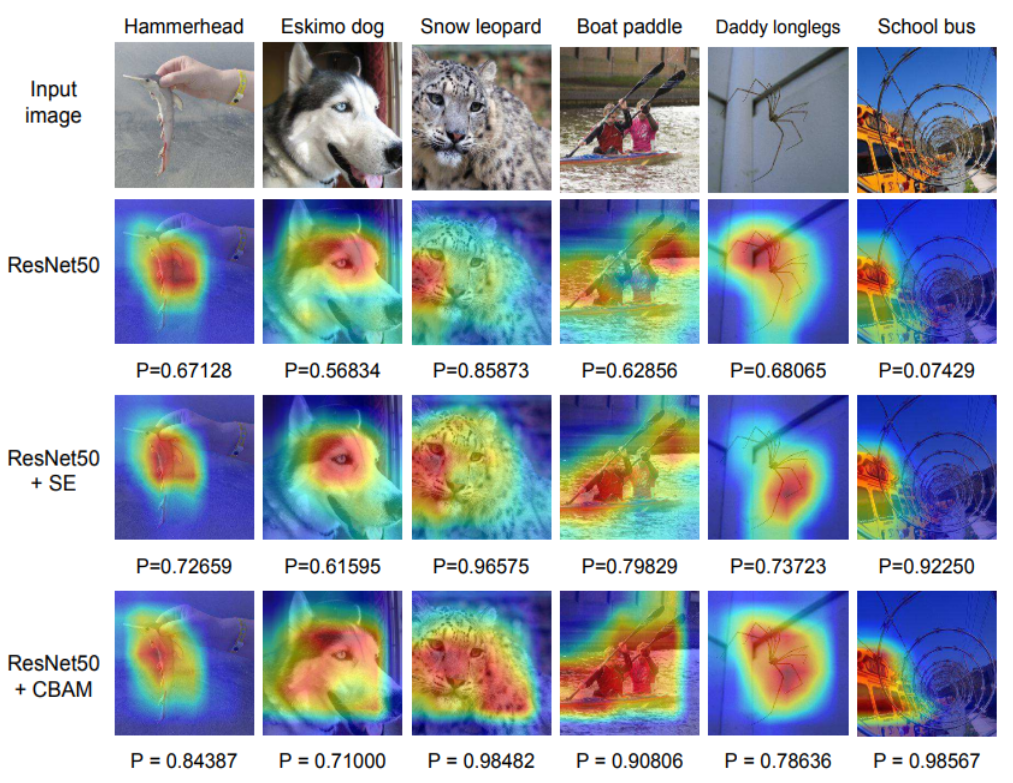
\includegraphics[width=0.8\linewidth]{images/attention.png}}
    \caption{Attention mechanism with highlighted areas \cite{wooCBAMConvolutionalBlock2018}}
    \label{fig:attention_diagram}
\end{figure}

Attention blocks are a component commonly used in deep neural networks to selectively focus on certain parts of the input data, allowing the model to prioritize important features and reduce noise in the input signal. Figure \ref{fig:attention_diagram} showcases this by displaying a Convolutional Block Attention Module which highlights most if not the entire object more accurately than other versions. Attention blocks have been used in a variety of different neural network architectures, including convolutional neural networks (CNNs), recurrent neural networks (RNNs), and transformer models, and have been shown to improve performance on a wide range of tasks, including image classification, machine translation, and speech recognition.

An attention block typically consists of three main components: a query matrix \(Q\), a key matrix \(K\), and a value matrix \(V\). These matrices, which are generated by applying different linear transformations to the input data, represent queries and keys of dimension \(d_k\), and values of dimension \(d_v\). The query matrix \(Q\) facilitates the computation of similarities between the input data and the elements in the key matrix \(K\). The similarity scores are subsequently utilized to determine the weights assigned to the corresponding values in the value matrix \(V\). The output matrix is then computed using the prescribed equation \cite{vaswaniAttentionAllYou2023}:
\[\text{Attention}(Q,K,V) = \text{softmax}(\frac{QK^T}{\sqrt{d_k}})V\]
The values are combined after weighting to produce an output that selectively focuses on the relevant parts of the input data.

In the context of YOLOv3, attention blocks can be implemented in the backbone network, which develops the feature maps. Specifically, attention blocks can be inserted in between convolutional layers to selectively attend to important parts of the feature maps. This can assist the network to better focus on object features and improve its detection performance.

Another way to implement attention blocks in YOLOv3 is to use them in the detection head, which predicts the bounding boxes, confidence scores, and class probabilities. Here, attention blocks can be used to weigh the extracted features from different scales of the feature pyramid, helping the network better localize objects at different scales.

The idea behind attention blocks is to create a set of learned weights that indicate how important each feature is to the output of the network. These weights can then be used to weight the features in a given layer, so that the model pays more attention to the most important features while ignoring those that are less important.

CBAM is integrated in all the convolutional layers except for the detection layers of the YOLO-BAM and DSCBAM models \cite{chakarDepthwiseSeparableConvolutions2020}.
